% !TeX TS-program = txs:///latexmk | txs:///view-log | txs:///view-pdf | txs:///convert
\documentclass{article}
\usepackage{tikzducks}

\usepackage{geometry}

\begin{document}

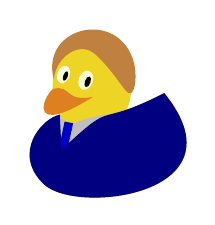
\begin{tikzpicture}
	\duck[tshirt=lightgray, 
			jacket=blue!50!black, 
			tie=blue!80!black, 
			shorthair]
\end{tikzpicture}
%

\begin{tikzpicture}
	\duck[santa=red!80!black, 
	      beard=white!80!brown]
\end{tikzpicture}
%

\begin{tikzpicture}
	\duck[graduate=gray!20!black,tassel=red!70!black]
\end{tikzpicture}	
%
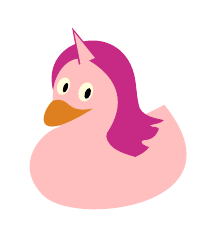
\begin{tikzpicture}
	\duck[body=pink,
		unicorn=magenta!60!violet,
		longhair=magenta!60!violet]
\end{tikzpicture}
%
\definecolor{fskin}{RGB}{161,140,126}%
\definecolor{fbill}{RGB}{238,212,191}%
\definecolor{fhair}{RGB}{89,72,72}%
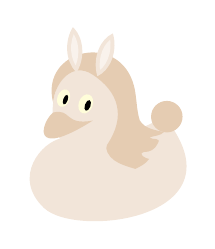
\begin{tikzpicture}
\duck[body=white!80!brown, bill=white!60!brown, bunny, longhair=white!60!brown]
\fill[white!60!brown] (1.85,1.42) circle (0.2);
\end{tikzpicture}
%
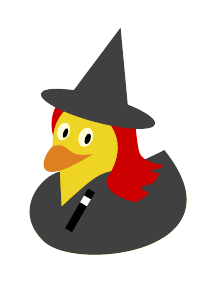
\begin{tikzpicture}
	\duck[witch=black!50!gray,
				longhair=red!80!black,
				jacket=black!50!gray,
				magicwand]
\end{tikzpicture}


\begin{tikzpicture}
	\duck[magichat,magicwand]
\end{tikzpicture}
%

\begin{tikzpicture}
	\duck[mask=teal,cape=teal]
\end{tikzpicture}
%
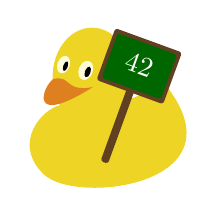
\begin{tikzpicture} 
    \duck[signpost=42]
\end{tikzpicture}
%

\begin{tikzpicture}
	\duck[lightsaber=red]
\end{tikzpicture}
%
\definecolor{qskin}{RGB}{225,219,206}%
\definecolor{qbill}{RGB}{170,123,154}%
\definecolor{qdress}{RGB}{184,209,206}%
\definecolor{qcrown}{RGB}{90,76,183}%
\begin{tikzpicture}
\duck[body=qskin,bill=qbill,jacket=qdress,tshirt=teal!30!qdress,shorthair=gray!60!white,necklace=gray!10!white,crown]  
\end{tikzpicture}
%

\begin{tikzpicture}
	\duck[icecream]
\end{tikzpicture}


\begin{tikzpicture}
	\duck[chef=white!85!gray,
			rollingpin=brown!80!black]
\end{tikzpicture}
%
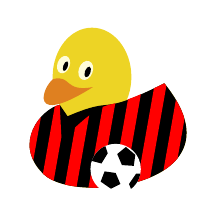
\begin{tikzpicture}
\duck[tshirt=black,stripes={\stripes[color=red]},football]
\end{tikzpicture}
%
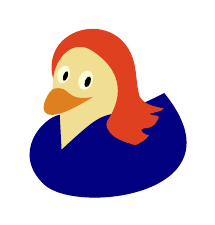
\begin{tikzpicture}
	\duck[body=yellow!50!brown!50!white, 
		longhair=red!50!brown, 
		jacket=blue!50!black]
\end{tikzpicture}
%

\begin{tikzpicture}
	\duck[cap,cricket]
\end{tikzpicture}
%

\begin{tikzpicture}
	\duck[body=yellow!50!brown!40!white,
		crazyhair=gray!50!white,
		eyebrow,
		glasses=brown!70!black,
		book=\scalebox{0.2}{$E=mc^2$},
		bookcolour=red!20!brown]
\end{tikzpicture}
%

\begin{tikzpicture}
	\duck[body=yellow!50!red!20!white,
		recedinghair=gray!50!white,
		eyebrow,
		tshirt=white!93!black,
		jacket=red!50!black,
		glasses=brown!70!lightgray,
		book=\scalebox{0.5}{\TeX},
		bookcolour=black!20!brown]
\end{tikzpicture}

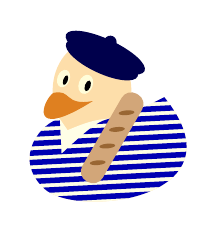
\begin{tikzpicture} 
\duck[body=yellow!60!red!30!white,tshirt=white!90!yellow,stripes={\stripes[color=blue!70!black,rotate=-87,width=0.07,distance=0.12]},beret=blue!30!black,baguette=brown]
\end{tikzpicture}
%
\definecolor{fskin}{RGB}{161,140,126}%
\definecolor{fbill}{RGB}{238,212,191}%
\definecolor{fhair}{RGB}{89,72,72}%
\begin{tikzpicture}
\duck[body=fskin,bill=fbill,shorthair=fhair,bunny,inear=fbill]
\node[fskin,rotate=45,scale=3] at (1.7,1.55) {\textsf{s}};
\fill[fhair,rotate=45] (2.4,0.13) ellipse (0.15 and 0.07); 
\end{tikzpicture}   
%

\begin{tikzpicture}
  \duck[cake=red!50!violet!80!black]
\end{tikzpicture}	
%
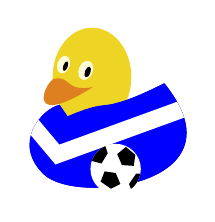
\begin{tikzpicture} 
\duck[tshirt=blue, jacket=blue,stripes={
	\stripes[color=white, rotate=-70, width=0.22,distance=1.1, initialy=0.01]
	\stripes[color=white, rotate=40, width=0.2, distance=1.8, initialy=1.0,initialx=0.285]
},football]
\end{tikzpicture}
%

\begin{tikzpicture}
	\duck[hockey=brown!70!black]
\end{tikzpicture}
%

\begin{tikzpicture}
	\duck[torch=black!30!gray]
\end{tikzpicture}


\end{document}

